\chapter{Applicazioni JavaEE}\label{app:javaee}
\begin{flushright}
	\parbox{13cm}{\small In questa appendice viene presentata la struttura di un'appilcazione web JavaEE, descrivendone le componenti ed il loro funzionamento. In particolare, viene descritto il funzionamento della servlet FacesServlet.}
\end{flushright}
\section{Panoramica}
JavaEE definisce un'architettura per lo sviluppo di servizi sotto forma di applicazioni multistrato, garantendo la scalabilità, l'accessibilità e la gestibilità necessarie per l'ambito aziendale. Il modello proposto suddivide il lavoro richiesto per l'implementazione di tali servizi in due parti:
\begin{itemize}
	\item la logica e la presentazione, a carico dello sviluppatore;
	\item i servizi standard, forniti dalla piattaforma JavaEE.
\end{itemize}
Lo sviluppatore può quindi fare affidamento sulla piattaforma per fornire soluzioni ai problemi di comunicazione con il sistema, derivanti proprio dalla struttura a più livelli del progetto.

\subsection{Struttura di un'applicazione distribuita}
Un'applicazione che utilizza JavaEE è composta da tre parti, presentati in \hyperref[fig:javaee-livelli]{figura \ref{fig:javaee-livelli}}:
\begin{itemize}
	\item \textbf{Client}: la prima parte è la macchina in cui l'utente finale utilizza l'applicazione. A questa è associato un livello omonimo, identificato con il browser e le pagine web in esso renderizzate.
	\item \textbf{JavaEE Server}: la seconda parte è il server. In esso risiedono due livelli:
	\begin{itemize}
		\item web: raggruppa i componenti necessari per la realizzazione di applicazioni web dinamiche, tra cui le pagine JSF e le servlet;
		\item \textit{business logic}: la logica dell'applicativo, sviluppata in Java.
	\end{itemize}
	\item \textbf{Database}: la terza parte (e livello) è quella che contiene i dati dell'applicazione. Può trovarsi su un server a sè stante o sullo stesso dove risiede l'applicazione JavaEE.
\end{itemize}
\begin{figure}
	\centering
	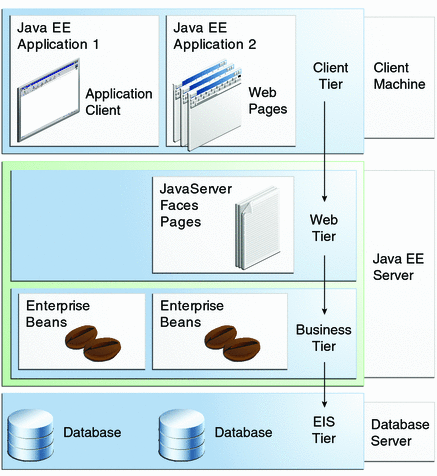
\includegraphics{Immagini/javaee-struttura.png}
	\caption{Struttura di un'applicazione distribuita JavaEE}
	\label{fig:javaee-livelli}
	\footnotesize\citetitle{bib:javaee-tutorial}. \citeauthor{bib:javaee-tutorial}. \citeyear{bib:javaee-tutorial}.
\end{figure}

\subsubsection{Componenti}
Ogni componente della JavaEE è un'unità software funzionale ed autonoma, che nel contesto globale dell'applicazione è in grado di interfacciarsi con gli altri componenti. In particolare, la specifica definisce i seguenti:
\begin{itemize}
	\item client applicativi e applet sono i componenti eseguiti a livello del client;
	\item Java Servlet, JavaServer Faces e JavaServer Pages sono i componenti web eseguiti sul server;
	\item \Gls{EJB} sono i componenti aziendali, la logica dell'applicazione, eseguiti sul server.
\end{itemize}

\subsubsection{Contenitori}
I contenitori sono l'interfaccia tra un componente e le funzionalità a basso livello dipendenti dalla piattaforma che il componente supporta. Ogni componente prima di essere eseguito deve essere assemblato in un modulo JavaEE e distribuito nel suo contenitore. 

Il processo di assemblaggio prevede la definizione delle configurazioni dei container per ciascun componente e per l'intera applicazione. Alcune delle configurazioni disponibili sono, ad esempio, il livello di accessibilità delle risorse (per limitare l'accesso ai soli utenti autorizzati), l'interfacciamento ai servizi ed il modello di connettività, per gestire a basso livello le comunicazioni tra i client e i \textit{bean}.

Un esempio di configurazione differente si ha impostando il tipo di distribuzione rispettivamente a \textit{development} o \textit{production}: nel primo caso, il comportamento dell'applicazione è mirato ad agevolare lo sviluppo, per esempio bloccando l'applicazione in caso di errori e stampando a video o nella \textit{console} vari log di tracciamento; a livello \textit{production}, invece, gli errori sono gestiti diversamente, con lo scopo di mantenere l'esecuzione fluida, senza creare disagi all'utente con messaggi a lui non comprensibili.

Esistono vari tipi di contenitori, che rispecchiano la struttura della piattaforma JavaEE:
\begin{itemize}
	\item contenitore EJB: gestisce l'esecuzione dei \textit{bean} sul server;
	\item contenitore web (es.: Tomcat): gestisce l'esecuzione di pagine web, servlet e dei \textit{bean} che si interfacciano con le pagine;
	\item contenitore client: gestisce l'esecuzione dei componenti client dell'applicazione.
\end{itemize}
La \hyperref[fig:javaee-contenitori]{figura \ref{fig:javaee-contenitori}} mostra le relazioni tra i contenitori.
\begin{figure}
	\centering
	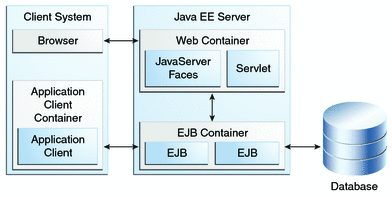
\includegraphics{Immagini/javaee-contenitori.png}
	\caption{Contenitori JavaEE}
	\label{fig:javaee-contenitori}
	\footnotesize\citetitle{bib:javaee-tutorial}. \citeauthor{bib:javaee-tutorial}. \citeyear{bib:javaee-tutorial}.
\end{figure}

\section{Applicazioni web JavaEE}
\subsection{Ciclo di vita}
Un'applicazione web consiste in componenti web, risorse statiche (es.: immagini), classi di supporto e librerie. Il contenitore web della JavaEE fornisce numerosi servizi che migliorano le funzionalità dei componenti e li rendono di fatto più semplici da implementare. Tuttavia, poiché un'applicazione web deve tener conto di questi servizi, il processo per la creazione e l'esecuzione di un'applicazione web è diverso da quello delle classi Java tradizionali e può essere riassunto in sei step:
\begin{enumerate}
	\item sviluppo del componente;
	\item sviluppo del \gls{descrittore di distribuzione} dell'applicazione, se necessario;
	\item compilazione dei componenti e delle classi di supporto;
	\item creazione di un pacchetto di distribuzione (opzionale);
	\item distribuzione dell'applicazione in un contenitore web;
	\item accesso ed utilizzo dell'applicazione tramite \Gls{URL}.
\end{enumerate}

\subsection{Struttura di un modulo web}
Nell'architettura Java EE, un modulo web è la più piccola unità distribuibile e utilizzabile. Esso contiene componenti e file di contenuto statici, quali immagini, che vengono definiti risorse web. Un modulo web JavaEE corrisponde ad un'applicazione web come definita nella specifica Java Servlet.

Il modulo web ha una struttura specifica, presentata in \hyperref[fig:javaee-modulo]{figura \ref{fig:javaee-modulo}}: la \textit{directory} di livello superiore è la radice del documento, in cui vengono memorizzate le pagine \texttt{XHTML}, le classi, gli archivi e le risorse. La radice contiene una sottodirectory denominata \texttt{WEB-INF}, che può contenere i seguenti elementi:
\begin{itemize}
	\item \texttt{classes}: una directory contenente le i file \texttt{.class}, risultato della compilazione del progetto;
	\item \texttt{lib}: una directory contenente i file \texttt{.jar} delle librerie richieste dall'applicazione;
	\item descrittori di distribuzione, come il file \texttt{web.xml}, descrittore dell'applicazione. Questo file è richiesto nel caso di utilizzo di JSF o se si vogliono specificare alcune configurazioni.
\end{itemize}

L'installazione del modulo nel contenitore web avviene tramite pacchetto WAR, che lo comprime e ne permette la distribuzione in qualsiasi contenitore web conforme alla specifica Java Servlet.

\begin{figure}
	\centering
	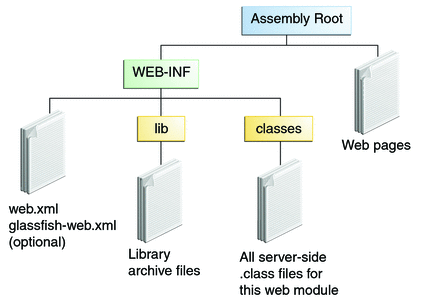
\includegraphics{Immagini/javaee-modulo.png}
	\caption{Struttura di un modulo web}
	\label{fig:javaee-modulo}
	\footnotesize\citetitle{bib:javaee-tutorial}. \citeauthor{bib:javaee-tutorial}. \citeyear{bib:javaee-tutorial}.
\end{figure}

\section{Servlet}
La tecnologia Java Servlet nasce per fornire contenuti dinamici ed orientati all'utente in modo indipendente dalla piattaforma. Deriva concettualmente dalla tecnologia CGI (Common Gateway Infrastructure), ma risolve i problemi di portabilità e scalabilità ad essa legati.

La servlet è una classe Java che estende le funzionalità del server che ospita l'applicazione, i cui accessi avvengono tramite un modello di programmazione \textit{request-response}. Sebbene le servlet possano rispondere a qualsiasi tipo di richiesta, sono di solito usate per estendere i server web. Esse processano le richieste e costruiscono le risposte, collegando il protocollo HTTP con il linguaggio Java.

\subsection{Ciclo di vita di una servlet}
Una servlet è gestita attraverso un ciclo di vita che definisce come viene caricata e istanziata, come viene inizializzata, come vengono gestite le richieste da parte dei client e infine come viene terminata. Il ciclo di vita è controllato dal contenitore in cui la servlet è stata installata.

Quando una richiesta viene mappata su una servlet, il contenitore esegue le seguenti operazioni:
\begin{enumerate}
	\item se non esiste un'istanza della servlet, il contenitore web
	\begin{enumerate}
		\item carica la classe;
		\item crea una istanza;
		\item inizializza l'istanza con il metodo \texttt{init};
	\end{enumerate}
	\item richiama il metodo \texttt{service} passandogli gli oggetti contenenti la richiesta e la risposta.
\end{enumerate}
Per rimuovere la servlet il container richiama il metodo \texttt{destroy}.